\documentclass{article}

\usepackage{amsmath,amssymb}
\usepackage{multicol}
\usepackage{systeme}
\usepackage{url}
%\usepackage{siunitx}

% for drawing graphs
\usepackage{tikz}
\tikzset{every picture/.style={thick}}
\tikzset{every node/.style={draw, circle, inner sep = 2pt}}
\usetikzlibrary{arrows}

% for margins
\usepackage[margin=1in]{geometry}

% for font
\usepackage{euler}
\usepackage[OT1]{eulervm}
\renewcommand{\rmdefault}{pplx}

\setlength{\parindent}{0pt}  %no indenting

% MACROS
\newcommand{\trans}{^\top}
\newcommand{\adj}{^{\rm adj}}
\newcommand{\cof}{^{\rm cof}}
\newcommand{\inp}[2]{\left\langle#1,#2\right\rangle}
\newcommand{\dunion}{\mathbin{\dot\cup}}
\newcommand{\bzero}{\mathbf{0}}
\newcommand{\bone}{\mathbf{1}}
\newcommand{\ba}{\mathbf{a}}
\newcommand{\bb}{\mathbf{b}}
\newcommand{\bd}{\mathbf{d}}
\newcommand{\be}{\mathbf{e}}
\newcommand{\bp}{\mathbf{p}}
\newcommand{\bq}{\mathbf{q}}
\newcommand{\bx}{\mathbf{x}}
\newcommand{\by}{\mathbf{y}}
\newcommand{\bz}{\mathbf{z}}
\newcommand{\bu}{\mathbf{u}}
\newcommand{\bv}{\mathbf{v}}
\newcommand{\bw}{\mathbf{w}}
\newcommand{\tr}{\operatorname{tr}}
\newcommand{\nul}{\operatorname{null}}
\newcommand{\rank}{\operatorname{rank}}
%\newcommand{\ker}{\operatorname{ker}}
\newcommand{\range}{\operatorname{range}}
\newcommand{\Col}{\operatorname{Col}}
\newcommand{\Row}{\operatorname{Row}}
\newcommand{\spec}{\operatorname{spec}}
\newcommand{\vspan}{\operatorname{span}}
% \newenvironment{sol}{\medskip\noindent {\bf Solution.}}{\newpage}
\newcommand{\mystrut}{\rule[-.5\baselineskip]{0pt}{2\baselineskip}}
% \newcommand{\mul}{\operatorname{mul}}
\newcommand{\even}{\operatorname{even}}
\newcommand{\sgn}{\operatorname{sgn}}
\newcommand{\iner}{\operatorname{iner}}
\newcommand{\rL}{\mathring{L}}
\newcommand{\diag}{\operatorname{diag}}

\makeatletter
%%%The definition of \binom is \genfrac ()\z@ {}
%%%To adjust the spaces between parantheses, change the augment of \kern
\newcommand{\multiset}[2]{\ensuremath{\left(\kern-.3em\left(\genfrac{}{}{\z@}{}{#1}{#2}\right)\kern-.3em\right)}}
\newcommand{\qanalog}[2]{\genfrac []\z@ {}{#1}{#2}_q}
\makeatother

% for title
\title{2021F Math585 Midterm1}
\date{\vspace{-1cm}}
\begin{document}
\maketitle
\large

\textbf{4 questions}, \textbf{20 total points}

\textbf{Note:}  Use other papers to answer the problems.  Remember to write down your \textbf{name} and your \textbf{student ID \#}.

\begin{enumerate}
\setlength\itemsep{2em}

\item{} [5pt] Let 
\[A = \begin{bmatrix}
 0 & x & 0 & 0 & 0 & 0 & 0 & 1 \\
 x & 0 & 1 & 0 & 0 & 0 & 0 & 0 \\
 0 & 1 & 0 & 1 & 0 & 0 & 0 & 0 \\
 0 & 0 & 1 & 0 & 1 & 0 & 0 & 0 \\
 0 & 0 & 0 & 1 & 0 & 1 & 0 & 0 \\
 0 & 0 & 0 & 0 & 1 & 0 & 1 & 0 \\
 0 & 0 & 0 & 0 & 0 & 1 & 0 & 1 \\
 1 & 0 & 0 & 0 & 0 & 0 & 1 & 0
\end{bmatrix}.\]
Find $x$ such that the $1,5$-entry of $A^4$ is $0$.

\item{} [5pt] Let $G$ be the Petersen graph and $A$ its adjacency matrix as shown below.

\begin{figure}[h]
\begin{center}
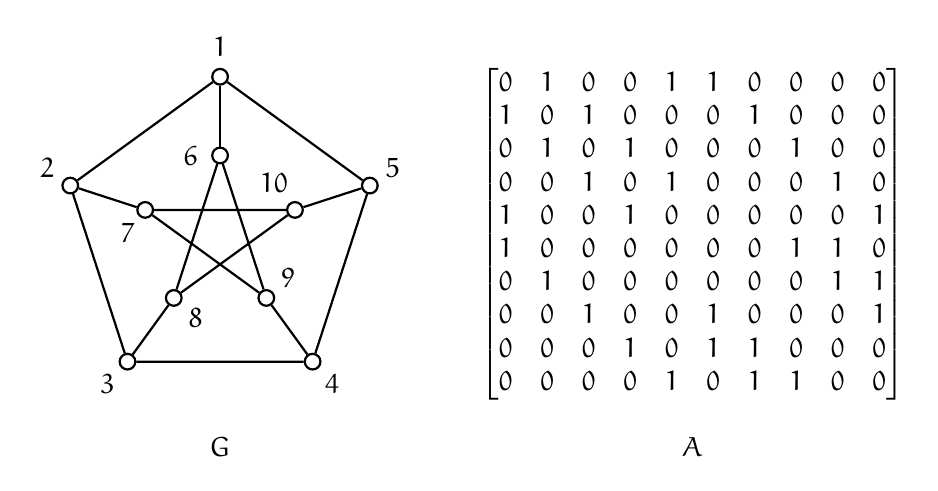
\begin{tikzpicture}
\begin{scope}[xshift=-3cm]
\foreach \i in {1,...,5} {
    \pgfmathsetmacro{\ang}{90 + 72*(\i - 1)}
    \node[label={\ang:$\i$}] (\i) at (\ang:2) {};
}
\foreach \i in {6,...,10} {
    \pgfmathsetmacro{\ang}{90 + 72*(\i - 6)}
    \pgfmathsetmacro{\j}{int(\i - 5)}
    \pgfmathsetmacro{\rang}{\ang + 90}
    \node[label={\rang:$\i$}] (\i) at (\ang:1) {};
    \draw (\i) -- (\j);
}
\draw (1) -- (2) -- (3) -- (4) -- (5) -- (1);
\draw (6) -- (8) -- (10) -- (7) -- (9) -- (6);
\node[below, rectangle, draw=none] at (0,-2.5) {$G$};
\end{scope}

\begin{scope}[xshift=3cm]
\node[rectangle,draw=none] at (0,0) {$\begin{bmatrix}
 0 & 1 & 0 & 0 & 1 & 1 & 0 & 0 & 0 & 0 \\
 1 & 0 & 1 & 0 & 0 & 0 & 1 & 0 & 0 & 0 \\
 0 & 1 & 0 & 1 & 0 & 0 & 0 & 1 & 0 & 0 \\
 0 & 0 & 1 & 0 & 1 & 0 & 0 & 0 & 1 & 0 \\
 1 & 0 & 0 & 1 & 0 & 0 & 0 & 0 & 0 & 1 \\
 1 & 0 & 0 & 0 & 0 & 0 & 0 & 1 & 1 & 0 \\
 0 & 1 & 0 & 0 & 0 & 0 & 0 & 0 & 1 & 1 \\
 0 & 0 & 1 & 0 & 0 & 1 & 0 & 0 & 0 & 1 \\
 0 & 0 & 0 & 1 & 0 & 1 & 1 & 0 & 0 & 0 \\
 0 & 0 & 0 & 0 & 1 & 0 & 1 & 1 & 0 & 0 \\
\end{bmatrix}$};
\node[below, rectangle, draw=none] at (0,-2.5) {$A$};
\end{scope}
\end{tikzpicture}
\end{center}
\end{figure}

Let $S_k$ be the sum of all $k\times k$ principal minors of $A$.  Find $S_5$ and explain your reasons.

\item{} [5pt] Let $J_n$ and $I_n$ be the $n\times n$ all-ones matrix and the identity matrix of order $n$, respectively.  Let $D_n = J_n - I_n$.  Find the inertia of $D_n$ and explain your reasons.

\vfill

\textbf{One more problem on the back.}

\newpage
\item{} [5pt] Let $A$ be a $7\times 7$ real symmetric matrix.  Let $\{\bv_1,\ldots, \bv_7\}$ be an orthonormal eigenbasis of $A$ such that $A\bv_i = \lambda_i\bv_i$ for $i = 1, \ldots, 7$ and $\lambda_1 \leq \cdots \leq \lambda_7$.  Consider the space $W = \vspan\{v_2,v_4,v_6\}$.  Show that 
\[\lambda_2 = \min_{\substack{\bx\in W\\\bx\neq\bzero}} \frac{\bx\trans A\bx}{\bx\trans\bx}.\]
\end{enumerate}



\end{document}



  
